\subsection{Singleton Pattern}

The singleton pattern \cite{GangOf4} ensures that a class has only one instance
and provides a global point of access to it. This is done by restricting access
to constructors so that other classes cannot create a new instance of a
singleton on its own. But if a class wants to use the singleton object instance,
it can use the singleton's static \verb!getInstance! method to obtain a
reference to the single instance.

\begin{figure}[t]
  \begin{center}
  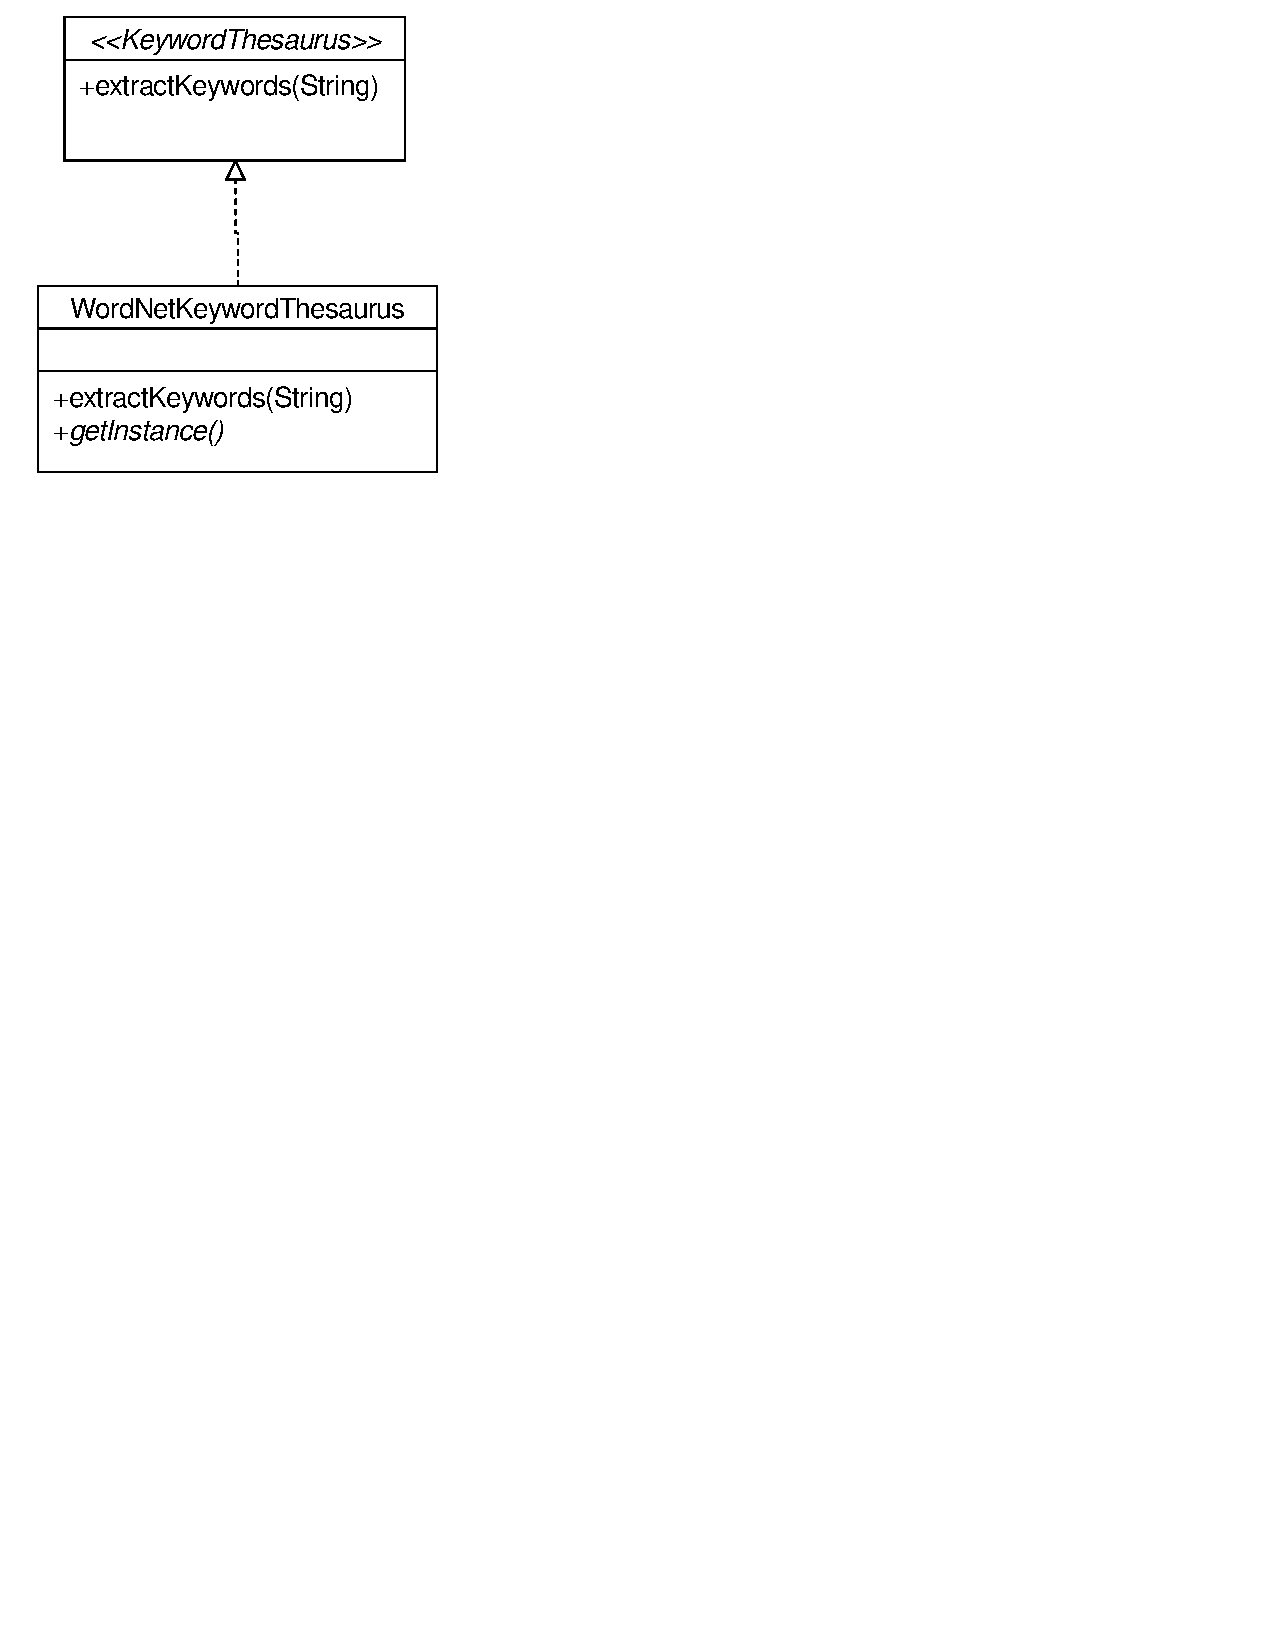
\includegraphics[scale=1.00]{images/singletonUML}
  \caption{Singleton UML in Coursebook}
  \label{fig:singletonUML}
  \end{center}
\end{figure}

The singleton design pattern is very simple. Figure \ref{fig:singletonUML} shows
how we use this design pattern in Coursebook. For most static utilities, like
the \verb!KeywordThesaurus!, it makes sense to use the singleton design pattern
because it saves memory and, for the context in which we use it, has no
concurrency side effects.

In Coursebook, our system has a utility interface called
\verb!KeywordThesaurus!. This interface takes an arbitrary string for input and
outputs a list of pertinent and similar keywords. Internally, the utility first
extracts the pertinent words from an arbitrary input, then identifies the part
of speech and generates a list of related words from the pertinent words. For
example, say a user's interest are: ``\textit{poetry and writing, travel,
skiing, flirting with the ladies}''. The keyword thesaurus will first prune this
input into this enumerated list: ``\textit{poetry, writing, travel, skiing,
flirting, ladies}''. The next phase of extraction will generate similar and
related words based on the pruned list: ``\textit{poetry, posey, verse, 
writing\_style, literary\_genre, writing, write, compose, travel, skiing, ski,
flirting, flirt, dally, coquet, coquette, romance, philander, ladies, lady, 
woman, girl}''. We obtain accurate and efficient results by combining both
keyword expansion and keyword extraction into a singleton object.

Since this algorithm is stateless and affects no other component of the system,
there are no multi-threading or concurrency issues. The singleton design pattern
is perfect for this utility because it eliminates the need to construct a new
\verb!KeywordThesaurus! object each time a client makes a request. This saves
memory because only one instance is needed.
